\subsection{Zielsetzung}

Das Hauptziel des Capacitor-NodeJS Plugins ist die Entwicklung eines Plugins für Capacitor, welches es Entwicklern ermöglicht, Node.js Projekte in Capacitor"=Anwendungen zu integrieren.
Um dies zu erreichen, soll eine Node.js Runtime eingebettet und gestartet werden, die das Ausführen eines Node.js Projektes übernimmt.

Das Plugin soll eine \ac{api} bereitstellen, um zwischen der Node.js Runtime bzw.\ dem Node.js Projekt und der Capacitor"=Anwendung zu kommunizieren.
Die \ac{api} soll an dem Node.js Event-Emitter angelehnt werden, um die Kompatibilität mit vorhandenen Node.js Projekten zu verbessern.

Das Plugin \textit{(und damit auch ein entsprechendes Node.js Projekt)} soll ohne zusätzlichen Aufwand sowohl in Mobile"=Anwendungen als auch in Desktop"=Anwendungen eingesetzt werden können.

\vspace{1em}

\begin{figure}[h]
  \centering
  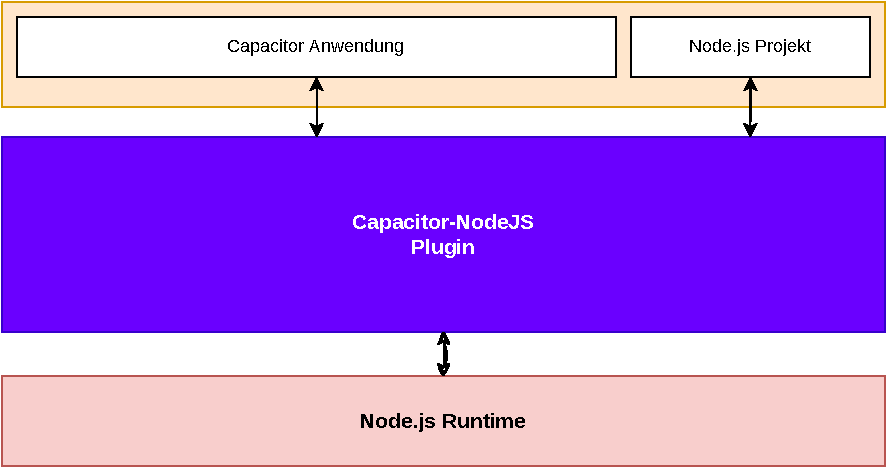
\includegraphics[width=0.8\textwidth]{assets/02_Capacitor-NodeJS/01_Zielsetzung.drawio.pdf}
  \caption[Capacitor-NodeJS / Zielsetzung]{Zielsetzung des Capacitor-NodeJS Plugins}
\end{figure}

Nachfolger von Node.js wie \enquote{Deno} oder \enquote{Bun} wurden in dieser Arbeit nicht berücksichtigt, da sie sich noch in einem frühen Stadium befinden und noch keine Unterstützung für Mobile"=Plattformen bieten.
\cite{deno, bun}

\begin{note}
  Die offizielle Entwicklungsumgebung für iOS, Xcode, ist ausschließlich für macOS verfügbar.~\cite{xcode:support}
  Da während der Entwicklung nur Windows- und Linux-Geräte zur Verfügung standen, war das Implementieren und Testen des Plugins für iOS nicht möglich.
\end{note}
